\begin{frame}{Digit Recognition using Deep Neural Network}
\begin{center}
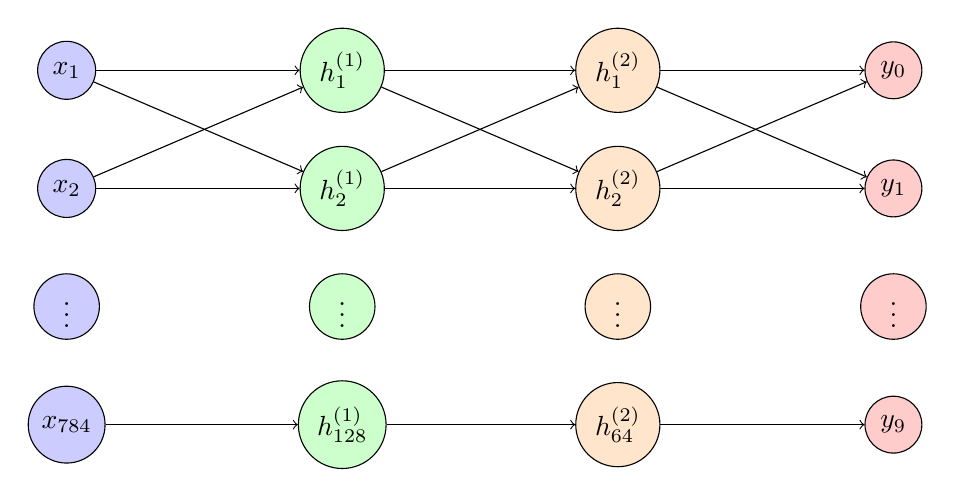
\begin{tikzpicture}[node distance=1.5cm]
    % Input layer
    \node[circle, draw, fill=blue!20] (i1) {$x_1$};
    \node[circle, draw, fill=blue!20, below of=i1] (i2) {$x_2$};
    \node[circle, draw, fill=blue!20, below of=i2] (i3) {$\vdots$};
    \node[circle, draw, fill=blue!20, below of=i3] (i4) {$x_{784}$};
    
    % First hidden layer
    \node[circle, draw, fill=green!20, right of=i1, xshift=2cm] (h1_1) {$h_1^{(1)}$};
    \node[circle, draw, fill=green!20, below of=h1_1] (h1_2) {$h_2^{(1)}$};
    \node[circle, draw, fill=green!20, below of=h1_2] (h1_3) {$\vdots$};
    \node[circle, draw, fill=green!20, below of=h1_3] (h1_4) {$h_{128}^{(1)}$};
    
    % Second hidden layer
    \node[circle, draw, fill=orange!20, right of=h1_1, xshift=2cm] (h2_1) {$h_1^{(2)}$};
    \node[circle, draw, fill=orange!20, below of=h2_1] (h2_2) {$h_2^{(2)}$};
    \node[circle, draw, fill=orange!20, below of=h2_2] (h2_3) {$\vdots$};
    \node[circle, draw, fill=orange!20, below of=h2_3] (h2_4) {$h_{64}^{(2)}$};
    
    % Output layer
    \node[circle, draw, fill=red!20, right of=h2_1, xshift=2cm] (o1) {$y_0$};
    \node[circle, draw, fill=red!20, below of=o1] (o2) {$y_1$};
    \node[circle, draw, fill=red!20, below of=o2] (o3) {$\vdots$};
    \node[circle, draw, fill=red!20, below of=o3] (o4) {$y_9$};
    
    % Connections
    \draw[->] (i1) -- (h1_1);
    \draw[->] (i1) -- (h1_2);
    \draw[->] (i2) -- (h1_1);
    \draw[->] (i2) -- (h1_2);
    \draw[->] (i4) -- (h1_4);
    
    \draw[->] (h1_1) -- (h2_1);
    \draw[->] (h1_1) -- (h2_2);
    \draw[->] (h1_2) -- (h2_1);
    \draw[->] (h1_2) -- (h2_2);
    \draw[->] (h1_4) -- (h2_4);
    
    \draw[->] (h2_1) -- (o1);
    \draw[->] (h2_1) -- (o2);
    \draw[->] (h2_2) -- (o1);
    \draw[->] (h2_2) -- (o2);
    \draw[->] (h2_4) -- (o4);
\end{tikzpicture}
\end{center}

\footnotesize
Deep neural network for digit recognition with 784 input neurons, 128+64 hidden neurons, and 10 output neurons
\end{frame}
